\chapter{State of the Art}
\label{sec:stateoftheart}

Machine learning research in amyotrophic lateral sclerosis (\gls{ALS}) covers several distinct tasks, including diagnosis, functional progression, survival, respiratory support, and patient stratification. These tasks are related, but they do not share the same target, prediction horizon, or evaluation requirements. This chapter therefore focuses on the literature most relevant to the two prognosis problems addressed in this dissertation: short-term functional progression and fixed-horizon survival. Particular attention is given to cohort construction, class imbalance, validation, reproducibility, and model interpretation.

\section{Clinical heterogeneity and prognostic outcomes}

\gls{ALS} is characterised by progressive degeneration of upper and lower motor neurons, but its course differs markedly between patients. Site and age of onset, diagnostic delay, respiratory function, nutritional status, and the initial pattern of functional impairment are all associated with prognosis~\cite{Feldman2022}. Median survival is commonly reported as two to four years from symptom onset, although a smaller group of patients survive substantially longer. A useful prognostic model must therefore describe variation between patients rather than only reproduce the average course of the disease.

Clinical follow-up relies heavily on the \gls{ALSFRS-R}, a 12-item scale covering bulbar, fine-motor, gross-motor, and respiratory function. Its total score provides a compact measure of disability, while its rate of change is often used to represent functional progression. Survival is a different outcome: it reflects the combined effect of disease progression, respiratory decline, nutritional complications, treatment, and supportive care. Models of functional decline and survival should consequently be compared within their own outcome definitions rather than treated as interchangeable measures of prognosis.

King's and MiToS staging translate clinical deterioration into ordered milestones, whereas the European Network for the Cure of ALS (ENCALS) model estimates individual survival groups from clinical predictors~\cite{Feldman2022}. Figure~\ref{fig:soa_figura1} summarises these complementary views of disease course. Staging is useful for describing a patient's current position; prognostic modelling asks what is likely to happen next and with what uncertainty.

\begin{figure}[ht!]
  \centering
  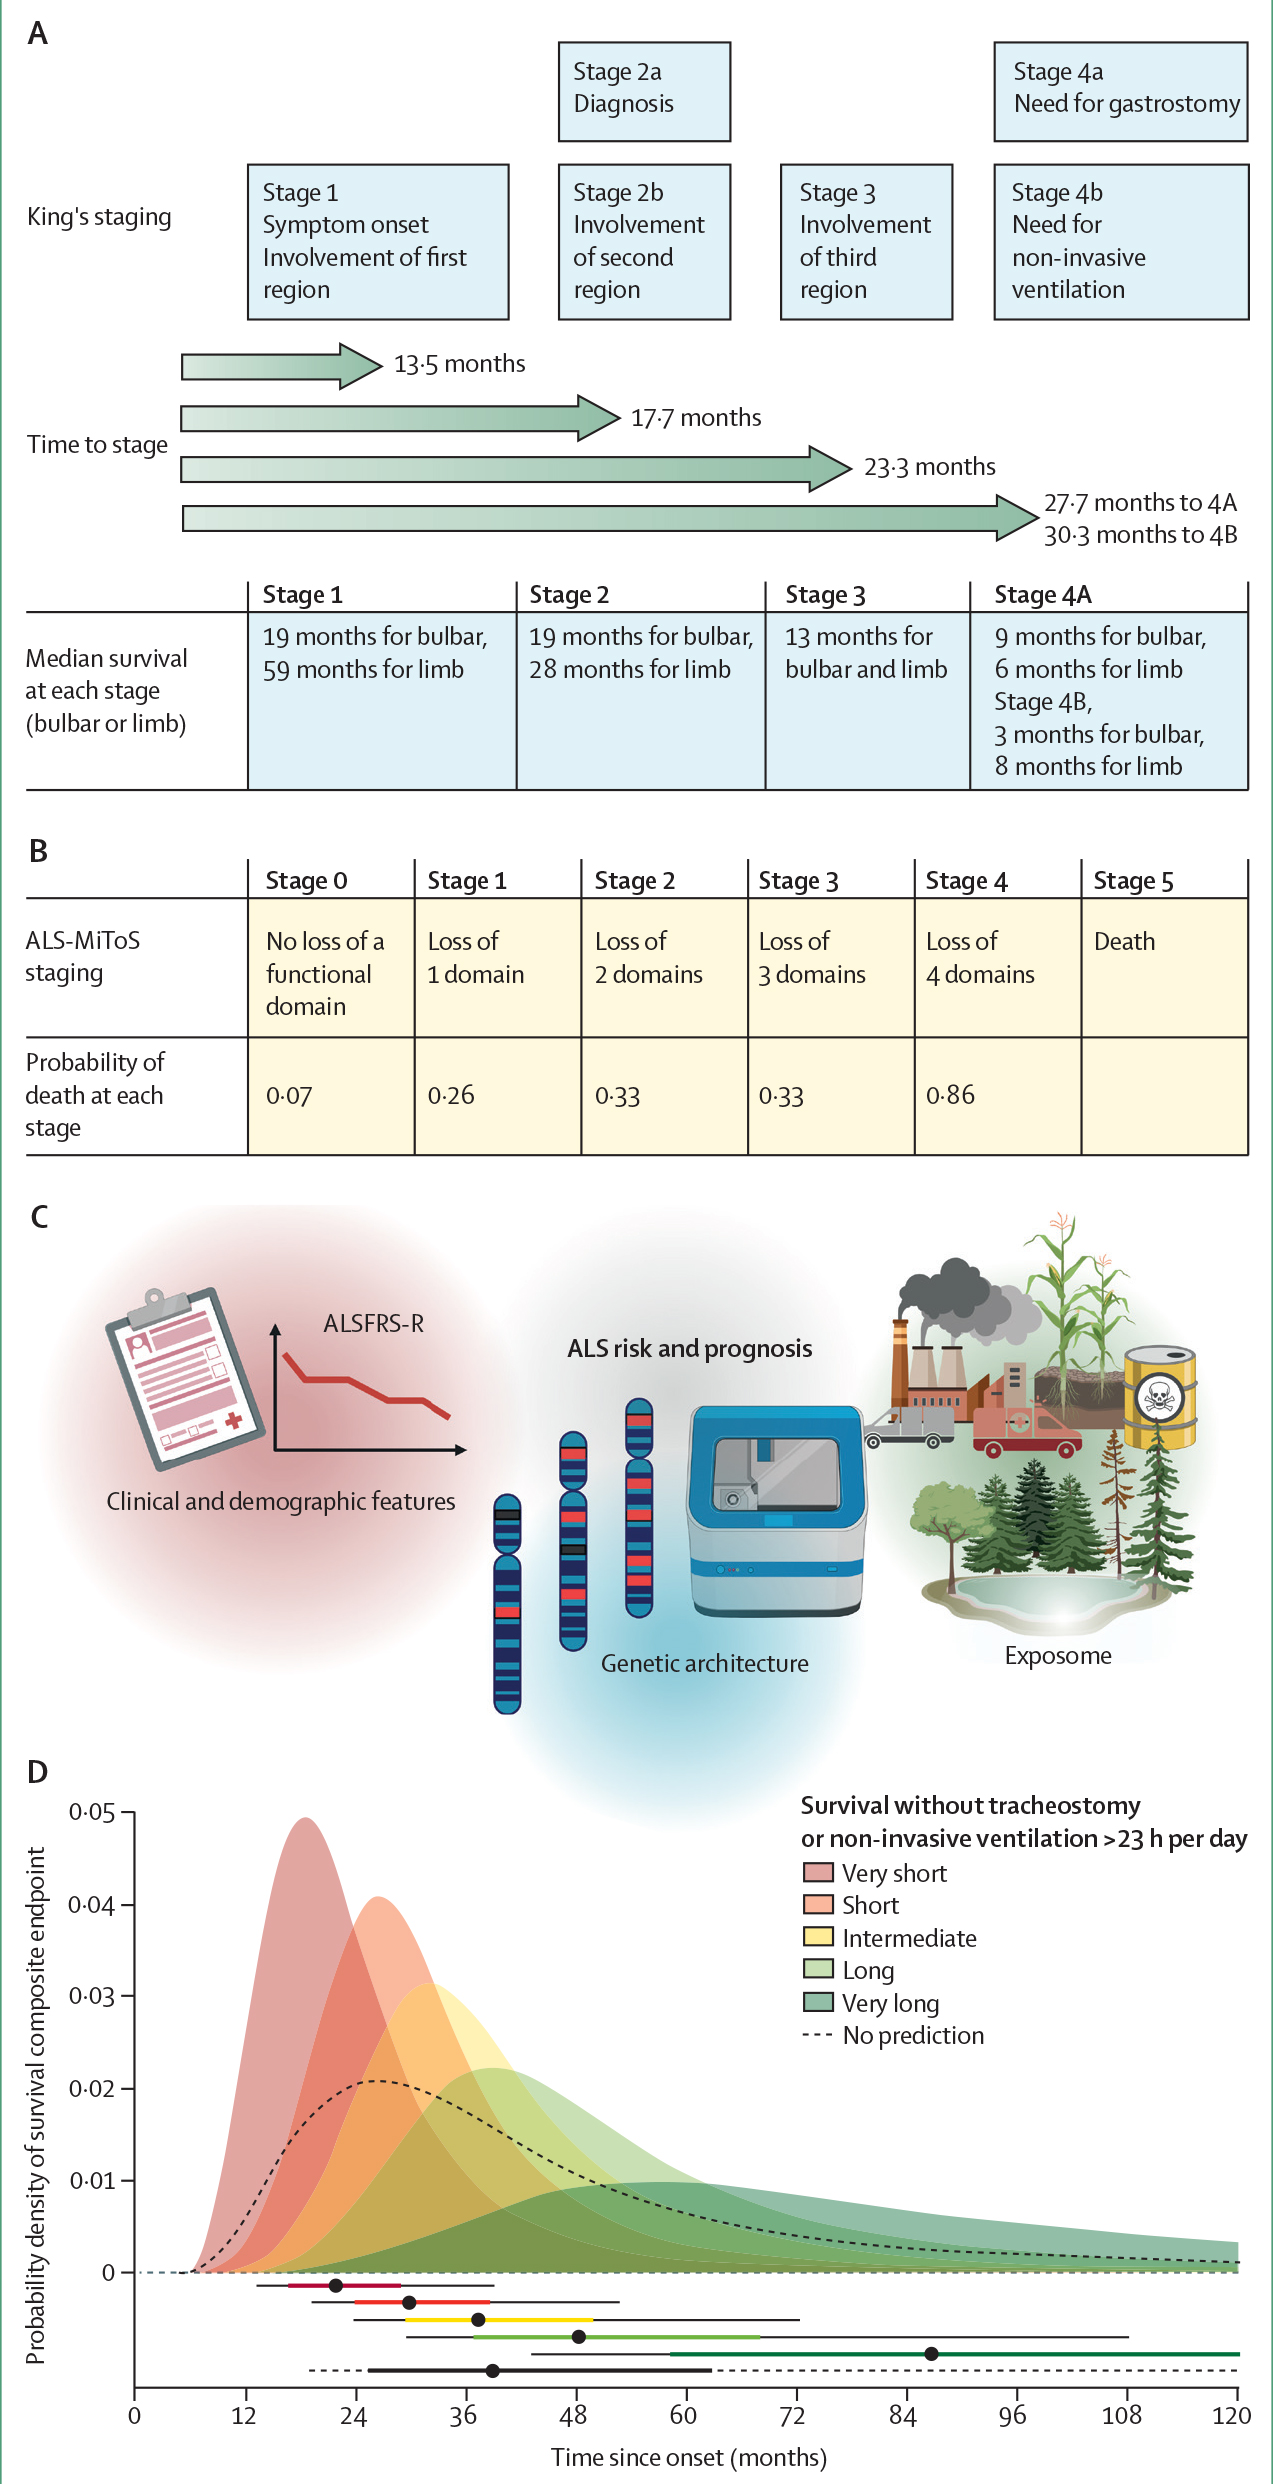
\includegraphics[width=0.65\linewidth]{./images/figures/figura1.jpg}
  \caption[ALS staging systems and survival groups]{Clinical descriptions of ALS progression and prognosis: King's staging, ALS-MiToS staging, factors associated with disease risk and outcome, and the ENCALS survival groups. Adapted from Feldman et al.~\cite{Feldman2022}.}
  \label{fig:soa_figura1}
\end{figure}

\clearpage
\section{Data sources, predictors, and outcome definitions}

The \gls{PRO-ACT} repository is the most frequently used public data source for ALS prognosis modelling. It pools records from clinical trials and includes longitudinal functional assessments, laboratory measurements, vital signs, respiratory tests, medication records, and survival information. Its size and accessibility support reproducible comparisons, and the DREAM Phil Bowen ALS Prediction Prize4Life Challenge established it as a benchmark for predicting later functional decline from early observations~\cite{Pancotti2022}.

The same properties that make \gls{PRO-ACT} useful also constrain the conclusions drawn from it. Trial eligibility criteria produce a selected population that is generally younger and less impaired than unselected clinical cohorts. Measurements are unevenly available across trials and follow-up becomes sparse over time. The final analytical cohort can therefore be much smaller than the number of registered patients, with its composition depending on the variables and observation window required by each study~\cite{Grollemund2019,Papaiz2022,Pancotti2022}. Performance within \gls{PRO-ACT} does not by itself establish performance in routine care.

Independent cohorts partly address this limitation. Registry, hospital, and trial-specific datasets such as ExonHit offer different patient populations and recording practices, although they are usually smaller and less accessible. Anani et al., for example, combined \gls{PRO-ACT} and ExonHit data when studying one-year survival and short-term functional progression~\cite{Anani2023}. Segura et al. used natural language processing to extract symptom onset, diagnosis, and subsequent clinical events from electronic health records for 250 patients across five Spanish hospitals~\cite{Paganoni2023}. Their work is not a prognosis model in the same sense as the \gls{PRO-ACT} studies, but it shows that real-world records can recover temporal information that is poorly represented in structured trial tables.

Across datasets, a relatively stable group of predictors appears: baseline \gls{ALSFRS-R}, its rate of decline, age at onset, diagnostic delay, site of onset, \gls{FVC}, \gls{BMI}, and creatinine~\cite{Grollemund2019,Papaiz2022}. Their repeated selection is clinically plausible, but it does not remove the need to examine how they were measured, when they became available, and whether missingness altered the cohort. A variable may be prognostic while still being unsuitable for a baseline model if its value is recorded after the intended prediction time.

\section{Functional progression prediction}

Functional prognosis is commonly formulated either as regression of a future \gls{ALSFRS-R} score or slope, or as classification into progression groups. The regression formulation preserves more information but produces errors in score units that may be difficult to translate into a clinical decision. Classification is easier to interpret, although it depends on a threshold that can change the class balance and the apparent difficulty of the task.

Figure~\ref{fig:soa_figura2} shows the distribution used by Pancotti et al. to separate fast from medium--slow progression. It also illustrates a general problem with dichotomised slopes: patients close to the boundary receive different labels despite having similar observed rates of decline. The threshold must therefore be reported together with the observation window and the method used to estimate each patient's slope.

\begin{figure}[ht!]
  \centering
  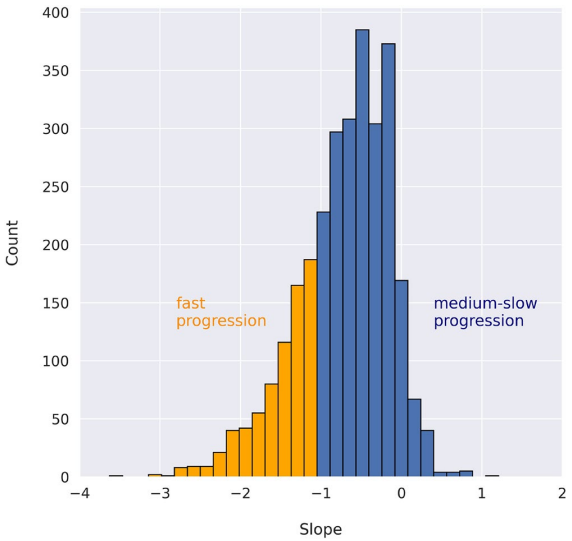
\includegraphics[width=0.45\linewidth]{./images/figures/figura2.png}
  \caption[ALSFRS-R slope distribution in PRO-ACT]{Distribution of ALSFRS-R slopes in the PRO-ACT cohort analysed by Pancotti et al. More negative values indicate faster functional decline; the colours show the study's division between fast and medium--slow progressors. Adapted from Pancotti et al.~\cite{Pancotti2022}.}
  \label{fig:soa_figura2}
\end{figure}

Early \gls{PRO-ACT} benchmarks showed that later decline could be estimated from demographic, functional, respiratory, and laboratory data. Subsequent work expanded the range of models from regression and random forests to boosting and deep neural networks~\cite{Grollemund2019,Papaiz2022}. The main gain has not been a single dominant algorithm. Rather, the literature shows that preprocessing, the definition of baseline, the amount of longitudinal history, and the evaluation split can affect performance as much as model family.

Pancotti et al. compared three deep-learning architectures that combined static and longitudinal \gls{PRO-ACT} data~\cite{Pancotti2022}. Their models achieved results comparable to established approaches, but no architecture held a clear advantage once uncertainty and differences in test design were considered. The authors also identified an apparent ceiling in slope prediction from the available variables. This is a more cautious conclusion than the common assumption that a more complex architecture will necessarily improve prognosis.

Anani et al. studied one-year survival alongside three-month \gls{ALSFRS} prediction using \gls{PRO-ACT} and ExonHit data~\cite{Anani2023}. They applied feature selection before fitting regression and classification models and reported an adjusted $R^2$ of 0.796 with a root mean squared error (RMSE) of 2.86 for the three-month functional outcome. As this work is a preprint, the result should be treated as preliminary, but it supports two useful points: compact feature sets can retain predictive signal, and functional and survival targets can be examined within the same patient representation without being conflated.

Qin et al. compared XGBoost, LightGBM, a one-dimensional convolutional network, and an ensemble on \gls{PRO-ACT}~\cite{Qin2025}. After tuning, the reported progression results were close: the deep model achieved $R^2=0.718$ and RMSE $=4.511$, while the ensemble produced $R^2=0.719$ and RMSE $=4.504$. Figure~\ref{fig:soa_figura3} presents the individual-model comparison. The small separation between models again suggests that model complexity was not the principal limitation.

\begin{figure}[ht]
  \centering
  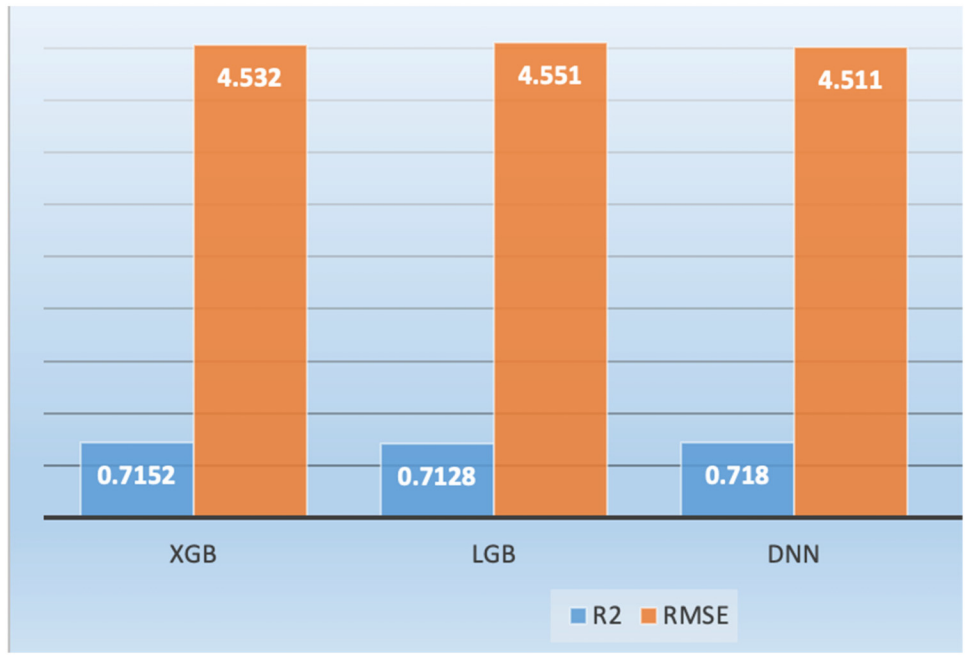
\includegraphics[width=0.85\linewidth]{./images/figures/figura3.png}
  \caption[Progression performance after model optimisation]{Reported $R^2$ and RMSE values for XGBoost, LightGBM, and a deep neural network after hyperparameter optimisation. The metrics use different scales and should be read separately. Adapted from Qin et al.~\cite{Qin2025}.}
  \label{fig:soa_figura3}
\end{figure}

\section{Survival prognosis}

Survival modelling ranges from time-to-event analysis to classification at a fixed horizon. Cox models and personalised survival tools such as ENCALS retain information about event timing and censoring. Fixed-horizon classification instead asks whether a patient will experience the event before a stated time, which produces a direct risk group but discards differences within each class. The choice should follow the intended use: estimating a survival curve and identifying short-survival patients are not the same statistical problem.

The review by Papaiz et al. found that ALS prognosis studies most often predicted functional progression, survival, or the need for interventions such as non-invasive ventilation and gastrostomy~\cite{Papaiz2022}. Survival studies repeatedly selected age, disease duration, functional status, respiratory measures, and nutritional indicators. Direct comparison remained difficult because cohorts, censoring rules, prediction horizons, and validation procedures differed across studies.

Papaiz et al. later developed a fixed-horizon model specifically for short-survival detection~\cite{Papaiz2024}. Their \gls{PRO-ACT} cohort contained 1,967 patients, of whom approximately 13\% died within 24 months of symptom onset. Six algorithms were evaluated: k-nearest neighbours, Naive Bayes, decision tree, random forest, \gls{SVM}, and neural network. Models were developed using five-fold cross-validation repeated three times within an 80\% training partition, followed by evaluation on a 20\% validation partition.

The study's principal contribution was an ensemble-imbalance design. Balanced Bagging was used for five classifiers and Balanced Random Forest for the random-forest model, with random undersampling applied inside the ensembles. Five of the six algorithm families improved significantly over their single-model counterparts after correction for multiple comparisons. The ensemble neural network achieved the strongest reported validation result, with balanced accuracy of 0.88, sensitivity of 0.96, and specificity of 0.80~\cite{Papaiz2024}. Papaiz et al. also used KernelSHAP to provide global and patient-level explanations for this model.

This design offers a clear replication target because the feature representation, survival definition, classifiers, resampling mechanism, and evaluation sequence are documented. It also leaves room for a broader methodological comparison. The reference study used grid search and one ensemble-level imbalance mechanism per classifier family. It did not compare individual over-sampling, under-sampling, and hybrid strategies, include LightGBM, report bootstrap confidence intervals, or analyse how decision thresholds affected short-survivor sensitivity. These are the extensions examined in Study~II.

\section{Longitudinal modelling and patient stratification}

Collapsing a patient's history into a baseline value or a linear slope simplifies modelling but can conceal changes in progression rate. Longitudinal methods instead estimate trajectories or latent patient groups from repeated measurements. Their practical difficulty is that ALS follow-up is irregular: patients enter studies at different disease stages, attend a different number of visits, and are increasingly likely to have missing observations as disease advances.

Ramamoorthy et al. addressed this setting with a mixture of Gaussian processes applied to sparse longitudinal data~\cite{Ramamoorthy2022}. The model identified non-linear progression patterns associated with differences in survival, showing that patient groups can be derived from temporal behaviour rather than imposed through a single slope threshold. Such groups may support trial stratification, but their stability must be checked across cohorts because clustering has no externally observed ``correct'' label.

Halbersberg and Lerner reviewed statistical, supervised, and unsupervised approaches to ALS progression and stratification~\cite{Halbersberg2023}. Their synthesis shows a recurring trade-off. Rich temporal models can represent dependencies between functional and respiratory domains, but they require denser follow-up and are harder to validate. Simpler baseline models apply to more patients and are easier to reproduce, at the cost of reducing the disease history to a small set of measurements. The two studies in this dissertation adopt the latter setting because their aim is risk estimation from information available near baseline or diagnosis.

\section{Class imbalance, metrics, and decision thresholds}
\label{sec:soa_imbalance}

Class imbalance is determined by the target definition rather than by the disease alone. A percentile-based rapid-progression target can be fixed near 30\% by design, whereas short survival within 24 months may represent little more than one patient in ten. The second setting gives a classifier more opportunities to achieve high overall accuracy by predicting the majority class, making accuracy unsuitable as the principal selection criterion.

Resampling and cost-sensitive learning address different parts of this problem. Class weights alter the penalty assigned to errors during training. Random under-sampling reduces the majority class, while \gls{SMOTE}, BorderlineSMOTE, and \gls{ADASYN} generate or emphasise minority examples. Hybrid methods such as \gls{SMOTEENN} and \gls{SMOTETomek} combine over-sampling with data cleaning~\cite{chawla2002smote,lemaitre2017}. None is uniformly preferable. Synthetic sampling can distort a small or heterogeneous minority class, while aggressive under-sampling may discard useful majority information. Resampling must also occur inside each training fold; applying it before cross-validation would allow synthetic or related observations to leak across partitions.

Metric choice follows the clinical error of interest. \gls{ROC-AUC} measures ranking across all possible thresholds and is useful for comparing discrimination, but it does not describe the classifications produced at a particular operating point. \gls{PR-AUC} concentrates on precision and recall for the positive class and is more informative when that class is uncommon. Balanced accuracy gives equal weight to sensitivity and specificity after a threshold has been chosen. Reporting these metrics together avoids treating ranking quality and minority-class detection as if they were equivalent.

The distinction matters because a model can have a high \gls{ROC-AUC} while showing poor sensitivity at the default threshold of 0.5. \gls{ROC-AUC} depends on the ordering of scores, not on whether those scores cross a fixed boundary. A model may rank most short survivors above standard survivors but assign both groups probabilities below 0.5. Threshold analysis is therefore part of evaluation rather than a cosmetic adjustment made after reporting the main result. The selected threshold should be derived from development data and then assessed once on the held-out partition.

\section{Validation, replication, and reproducibility}

Validation design determines which claim a performance estimate can support. When several visits from one patient are available, record-level random splitting allows correlated observations to appear in both training and test data. Subject-level separation is required if the intended use is prediction for a previously unseen patient. Preprocessing, imputation, feature selection, resampling, and target thresholds must likewise be fitted without access to the held-out data~\cite{Grollemund2019,Papaiz2022}.

Cross-validation is not inherently weaker than a single holdout. Nested or properly separated cross-validation can provide a sound estimate, especially in small cohorts. The problem arises when the same folds influence feature selection, hyperparameter tuning, model selection, and final reporting without accounting for that repeated use. A sealed test partition offers a separate final check, although its estimate may be imprecise when the minority class is small. Confidence intervals and the underlying confusion matrix are then needed to show that uncertainty.

External validation asks whether a model transfers to a different population. Reproducibility asks whether the same analysis can be rerun from the reported data and methods. Replication goes further by testing whether the central conclusion survives an independent implementation or a changed experimental design. These questions are often merged under the term ``validation'', but they expose different weaknesses. A fully reproducible \gls{PRO-ACT} result may still fail in a hospital cohort, while an externally tested model may be impossible to recreate from its publication.

The Papaiz et al. study is suitable for replication because it uses a public data source and specifies the target, feature set, model families, imbalance mechanism, and evaluation procedure~\cite{Papaiz2024}. Study~II first tests its central claim that imbalance-aware ensembles improve short-survival classification. It then changes selected components---optimisation, classifier set, resampling strategy, uncertainty estimation, and threshold analysis---to determine which conclusions remain stable. This framing is narrower and more defensible than claiming that replication of ALS machine learning has previously been absent.

\section{Explainability in ALS prognosis}

Interpretability can be introduced through the model itself or through a post-hoc explanation method. Regression coefficients, shallow trees, and compact feature sets expose part of the decision structure directly. More flexible models require additional tools to describe how features influence predictions. In both cases, an explanation concerns the fitted model; it does not establish that a feature causes the clinical outcome.

Feature selection is one route to simpler models. Anani et al. used feature selection before ridge-based survival prediction and functional regression, reducing the number of variables considered by the final models~\cite{Anani2023}. The benefit is not automatic. A smaller set is easier to inspect, but its stability across folds and cohorts matters more than the number of retained variables.

Pancotti et al. applied SHAP to their deep progression models and found contributions from functional subscores, time from onset to diagnosis, respiratory measurements, and creatinine~\cite{Pancotti2022}. Figure~\ref{fig:soa_figura4} shows the distribution of feature contributions across patients. Papaiz et al. used KernelSHAP for their ensemble neural network, including both global rankings and local explanations of individual survival classifications~\cite{Papaiz2024}. These studies show that post-hoc explanation is already present in ALS prognosis research; the remaining question is whether explanations are stable, clinically coherent, and evaluated beyond a visual example.

\clearpage
\begin{figure}[ht]
  \centering
  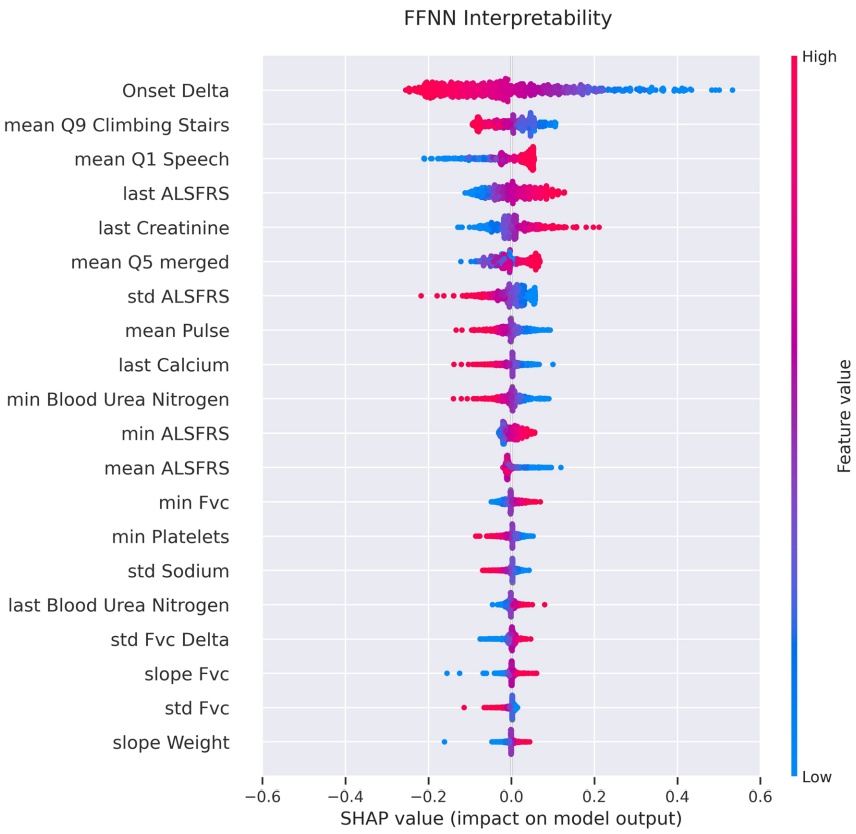
\includegraphics[width=0.80\linewidth]{./images/figures/figura4.png}
  \caption[SHAP feature contributions in progression prediction]{SHAP summary for a progression model reported by Pancotti et al. Each point is one patient; position gives the direction and magnitude of the model contribution, while colour represents the observed feature value. Adapted from Pancotti et al.~\cite{Pancotti2022}.}
  \label{fig:soa_figura4}
\end{figure}

Explanation quality is constrained by the data and experimental design. Correlated variables can divide or exchange attribution, missingness indicators may become proxies for trial procedures, and a plausible ranking does not validate the prediction itself. For this reason, the explainability analyses in this dissertation are interpreted alongside held-out performance and are described as predictive associations rather than causal findings.
\clearpage
\section{Comparison of representative studies}

Table~\ref{tab:soa_comparison} summarises the studies most closely related to the dissertation. The comparison separates outcome, data, modelling, and evaluation because similar algorithm names can conceal substantially different prediction tasks.

\begin{table}[ht!]
\centering
\caption[Representative ALS prognosis studies]{Representative studies related to functional progression, survival prognosis, and longitudinal stratification.}
\label{tab:soa_comparison}
\small
\resizebox{\textwidth}{!}{%
\begin{tabular}{p{2.5cm} p{2.4cm} p{3.0cm} p{3.4cm} p{4.3cm}}
\toprule
\textbf{Study} & \textbf{Data} & \textbf{Outcome} & \textbf{Approach} & \textbf{Relevant observation} \\
\midrule
Pancotti et al.~\cite{Pancotti2022} &
\gls{PRO-ACT} &
\gls{ALSFRS-R} slope and progression group &
Three deep architectures using static and longitudinal inputs &
Deep models were comparable with established methods; SHAP was used to examine feature contributions. \\

Ramamoorthy et al.~\cite{Ramamoorthy2022} &
Multiple longitudinal cohorts &
Progression trajectories and associated survival &
Mixture of Gaussian processes &
Non-linear trajectory groups can be recovered from sparse follow-up, but cohort transfer remains important. \\

Anani et al.~\cite{Anani2023} &
\gls{PRO-ACT} and ExonHit &
One-year survival and three-month functional score &
Feature selection with regression and classification models &
Compact models retained predictive signal; results are reported in a non-peer-reviewed preprint. \\

Papaiz et al.~\cite{Papaiz2024} &
\gls{PRO-ACT} ($N=1{,}967$) &
Death within 24 months of symptom onset &
Six classifiers with imbalance-aware ensembles &
The ensemble neural network reached 0.88 balanced accuracy; evaluation included a separate 20\% validation partition and KernelSHAP. \\

Qin et al.~\cite{Qin2025} &
\gls{PRO-ACT} &
Functional progression and onset type &
XGBoost, LightGBM, 1D CNN, and ensemble &
Optimised progression models produced similar $R^2$ and RMSE values, limiting claims of a clear architectural advantage. \\
\bottomrule
\end{tabular}%
}
\end{table}

\section{Research gaps and implications for this dissertation}
\label{sec:soa_synthesis}

The literature supports prediction from routinely collected ALS data, but four gaps remain directly relevant to this dissertation.

First, outcome construction is often treated as a minor preprocessing step even though it determines the cohort and class balance. Functional-progression labels depend on the follow-up window, slope estimator, and cut-off. Fixed-horizon survival labels depend on the time origin, censoring rule, and evidence that a patient survived beyond the horizon. Study~I therefore defines progression labels within the training procedure, while Study~II reconstructs the reference study's 24-month survival target before testing extensions.

Second, reported performance is difficult to compare when patient separation and tuning procedures differ. The literature contains sound validation designs, but reporting is not always sufficient to determine whether preprocessing and model selection were isolated from the final evaluation. Both studies in this dissertation reserve subjects before model development and keep the final partition outside optimisation. Study~I additionally computes the percentile-based progression threshold from training data rather than from the complete cohort.

Third, class imbalance requires more than selecting a single headline metric. Functional progression in Study~I has a moderate 30/70 split and is optimised using \gls{PR-AUC}. Short survival in Study~II is substantially rarer; the replication retains \gls{ROC-AUC} for ranking comparisons but also reports sensitivity, specificity, balanced accuracy, confusion matrices, and threshold behaviour. The two studies use different metrics because they answer different questions, not because one metric is universally superior.

Fourth, explainability is increasingly present in ALS modelling, but visual feature rankings are often presented without testing their stability or separating association from causation. Study~I combines SHAP and \gls{LIME} for functional-progression classification, while Study~II applies architecture-appropriate SHAP explainers to survival models. In both cases, explanations are used to inspect model behaviour after predictive performance has been established.

Study~I provides the dissertation's original functional-progression pipeline: baseline prediction, patient-level separation, fold-specific target construction, Bayesian optimisation, and held-out explanation. Study~II moves from model development to replication. It tests the published benefit of imbalance-aware ensembles and then broadens the comparison to LightGBM, ten individual resampling strategies, bootstrap uncertainty, and threshold analysis. Together, the studies examine two different ALS prognosis outcomes under a common set of requirements: explicit outcome construction, separated validation, imbalance-aware evaluation, reproducibility, and cautious interpretation.
